\chapter{Ανάλυση Απαιτήσεων Συστήματος}

\section{Λειτουργικές Απαιτήσεις}
\subsubsection{Έξοδοι του Συστήματος}
Στο σύστημα, αποδέκτες των εξόδων αποτελούν όλοι οι χρήστες του, δηλαδή οι πελάτες, οι καμαριέρες 
και καθώς και ο υπάλληλος υποδοχής. Παρακάτω αναγράφονται επιγραμματικά τα στοιχεία εξόδου 
ανάλογα με τον αποδέκτη του. 

\noindent \\ 
Στον πελάτη παρέχονται οι παρακάτω έξοδοι:
\begin{itemize}
	\item  Λίστα με προσφερόμενα γεύματα.
	\item  Λίστα πληροφοριών για την πόλη των Χανίων.
	\item  Προβολή ερωτήσεων που δέχεται από τον υπεύθυνο υποδοχής.
	\item  Προβολή απαντήσεων  που δέχεται από τον υπεύθυνο υποδοχής.		
	\item  Pop-up window κατά την αναμονή έγκρισης/απόρριψης της παραγγελίας.
\end{itemize}

\noindent \\
Στον υπάλληλο υποδοχής παρέχονται οι παρακάτω έξοδοι:
\begin{itemize}
	\item  Pop-up window σχετικά με την επεξεργασία των FAQ
	\item Προβολή ερωτήσεων που δέχεται από τον υπεύθυνο υποδοχής.
	\item Προβολή απαντήσεων  που δέχεται από τον υπεύθυνο υποδοχής.	
\end{itemize}

\noindent \\ 
Στις καμαριέρες παρέχονται οι παρακάτω έξοδοι:
\begin{itemize}
	\item  Pop-up window σχετικά με το αίτημα γεύματος από πελάτη.
	\item  Pop-up window σχετικά με την ολοκλήρωση  επαρκούς αριθμού δωματίων που καθαρίστηκαν.
\end{itemize}

\noindent \\ 
Ως αυτοματοποιημένη έξοδος, παρέχεται η εξής:
\begin{itemize}
	\item  Ανανέωση λίστας αντικειμένων προς ανανέωση
\end{itemize}

\begin{table}[H]
	\resizebox{\textwidth}{!}{%
		\begin{tabular}{|c|c|c|c|c|c|}
			\hline
			\textbf{Έξοδος}       & \begin{tabular}[c]{@{}c@{}}Pop-up window \\ κάθε είδους\end{tabular} & Λίστες Πληροφοριών & Ερωτήσεις  & Απαντήσεις   & \begin{tabular}[c]{@{}c@{}}Λίστα\\ αντικειμένων\end{tabular} \\ \hline
			\textbf{Τύπος Εξόδου} & Γραφική Διεπαφή                                                      & Γραφική Διεπαφή    & Απλό κείμενο & Απλό κείμενο & \begin{tabular}[c]{@{}c@{}}Αρχείου τύπου\\ .csv\end{tabular} \\ \hline
		\end{tabular}%
	}
\end{table}
\clearpage

\noindent\\
Αναφορικά με τον λόγο που παράγεται κάθε έξοδος, η προβολή ερωτήσεων και απαντήσεων
μεταξύ δύο χρηστών παράγεται μετά την έναρξη προσωπικής συνομιλίας από έναν χρήστη. Τα pop-up
Windows, παράγονται από τον πελάτη κατά την παραγγελία φαγητού ώστε να τον ενημερώσουν για
την έγκριση ή την απόρριψη της παραγγελίας του, στην καμαριέρα ώστε να εγκρίνει ή να  απορρίψει 
μία παραγγελία αλλά και στις περιπτώσεις όπου συμπλήρωσε τον απαιτούμενο αριθμό δωματίων τα 
οποία καθάρισε και στον υπάλληλο υποδοχής εφόσον επιτυχώς ενημέρωσε την λίστα με τις 
συχνές ερωτήσεις. Ακόμα, οι λίστες παράγονται σε περίπτωση που ο πελάτης θελήσεις να πληροφορηθεί 
σχετικά με τα Χανιά  ή στην περίπτωση που αιτηθεί παραγγελία γεύματος όπου και εμφανίζεται μία λίστα
με τα προσφερόμενα γεύματα. Τέλος, η αυτοματοποιημένη έξοδος που αναγράφεται, αναφέρεται στην 
αυτοματοποιημένη λειτουργία κατά την οποία το πρόγραμμα προσθέτει αντικείμενα στην λίστα 
παραγγελιών  του καταλύματος εαν βρεθεί πως υπάρχει έλλειψη μετά από έλεγχο των δεδομένων που 
εισήγαγε η καμαριέρα κατά τον καθαρισμό του δωματίου.\\

\noindent
Όσον αφορά τη γραφική διεπαφή pop-up window, είναι ένα παράθυρο τύπου pop-up στο οποίο εμφανίζεται
ένα μήνυμα σχετικό με το λόγο που παράχθηκε σε κάθε περίπτωση καθώς και ένα ή δύο κουμπιά για την 
υλοποίηση επιμέρους διαδικασιών. Ενδεικτικά, στην περίπτωση έγκρισης παραγγελίας, αναγράφονται τα 
ζητούμενα γεύματα και υπάρχουν δύο κουμπιά με τα οποία μπορεί να εγκρίνει ή να απορρίψει της. 


\subsubsection{Είσοδοι του Συστήματος}
Οι είσοδοι του συστήματος χωρίζονται ανάλογα με το είδος του χρήστη. Λόγω της φύσης του 
συστήματος, οι χρήστες του συστήματος είναι οι πελάτες του καταλύματος, ο υπεύθυνος υποδοχής 
καθώς και οι καμαριέρες και ο κάθε ένας έχει τη δυνατότητα εκτέλεσης διαφορετικών διαδικασιών και ως
αποτέλεσμα, εισαγωγή διαφορετικών εισόδων σε αυτό.  Λόγω της φύσης του συστήματος, όλες οι 
είσοδοι προσλαμβάνονται από το σύστημα μέσω της οθόνης αφής κάθε συσκευής και στις περιπτώσεις
όπου απαιτείται η εισαγωγή κειμένου ή αριθμών, μέσω του πληκτρολογίου που εμφανίζεται σε αυτή.

\noindent \\ 
Στον πελάτη παρέχονται οι παρακάτω είσοδοι:
\begin{itemize}
	\item Σύνταξη μηνύματος ως ερώτηση σε προσωπική συνομιλία
	\item Σύνταξη μηνύματος ως απάντηση σε προσωπική συνομιλία
	\item Επιλογή γεύματος καθώς και αντίστοιχων πληροφοριών που ζητούνται κατά την παραγγελία
\end{itemize}

\noindent \\ 
Στον υπάλληλο υποδοχής παρέχονται οι παρακάτω είσοδοι:
\begin{itemize}
	\item Αλλαγή περιεχομένου FAQ
	\item Σύνταξη μηνύματος ως ερώτηση σε προσωπική συνομιλία
	\item Σύνταξη μηνύματος ως απάντηση σε προσωπική συνομιλία 
\end{itemize}

\noindent \\ 
Στην καμαριέρα παρέχονται οι παρακάτω είσοδοι:
\begin{itemize}
	\item Απόρριψη ή έγκριση παραγγελίας πελάτη
	\item Συμπλήρωση πλήθους αντικειμένου κάθε δωματίου
\end{itemize}


\subsubsection{Προτεραιότητες και Διαδικασίες του Συστήματος}
Το σύστημα έχει 6 προβλεπόμενες διαδικασίες οι οποίες φαίνονται στο παρακάτω High level use case 
διάγραμμα \ref{high_level_use_case}  
\begin{figure}[H]
	\centering
	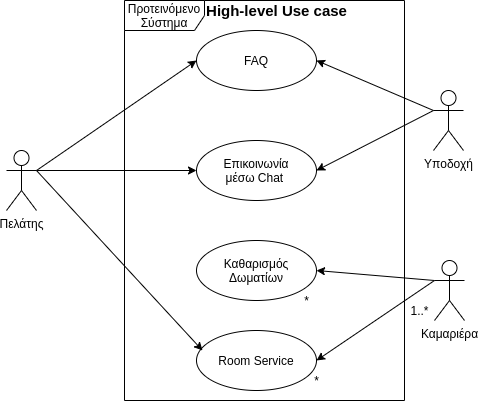
\includegraphics[width=0.7\textwidth]{Images/High_level_use_case}
	\caption{High Level Use Case Diagram}
	\label{high_level_use_case}
\end{figure}

\noindent
Οι επιμέρους διαδικασίες περιγράφονται στη συνέχεια συνοδευόμενες από διαγράμματα σχετικά 
με την κάθε μία. Πιο συγκεκριμένα, έχουν κατασκευαστεί τα Detailed use case διαγράμματα  καθώς 
και τα actor action - System event διαγράμματα για κάθε διαδικασία ενώ για τις διαδικασίες "Room 
service" και "Επικοινωνία μέσω  Chat" έχουν δημιουργηθεί  τα αντίστοιχα Activity diagrams, για τις 
διαδικασίες  "FAQ" και  Καθαρισμός Δωματίων" έχουν δημιουργηθεί  τα Sequence diagrams και 
??????εεε και τα άλλα 2 όπως αυτά φαίνονται παρακάτω.\\

\noindent
Όσον αφορά την λειτουργία "Συχνών Ερωτήσεων" (FAQ) προβλέπονται δύο διαδικασίες που μπορούν να 
εκπονηθούν. Εμπλεκόμενοι σε αυτή τη λειτουργία είναι ο πελάτης και ο υπάλληλο υποδοχής. Όσον αφορά 
τον πελάτη, αρχικά, γίνεται η επιλογή της λειτουργίας "FAQ" στο κεντρικό μενού και στη συνέχεια 
εμφανίζεται στον χρήστη μία λίστα με ερωτήσεις μαζί με τις απαντήσεις τους, από τις οποίες μπορεί να 
αντλήσει χρήσιμες πληροφορίες. Όσον αφορά τον υπάλληλο υποδοχής, αρχικά, γίνεται η επιλογή της 
λειτουργίας "Επεξεργασίας FAQ" στο κεντρικό μενού και στη συνέχεια δίνεται η δυνατότητα Προσθήκης 
Επεξεργασίας/Διαγραφής μίας ερώτησης ή της αντίστοιχης απάντησης της από την λίστα. Με την 
ολοκλήρωση  της επεξεργασίας, εμφανίζεται το αντίστοιχο  pop-up window που τον ενημερώνει για 
την επιτυχή επεξεργασία των FAQ. Τέλος, η συγκεκριμένη διαδικασία παρουσιάζει χαμηλή προτεραιότητα
καθώς δεν αποτελεί σύγχρονη επικοινωνία μεταξύ χρηστών αλλά απλή παρουσίαση ήδη καταχωρημένων
πληροφοριών σε μορφή κειμένου.\\
\begin{figure}[H]
	\centering
	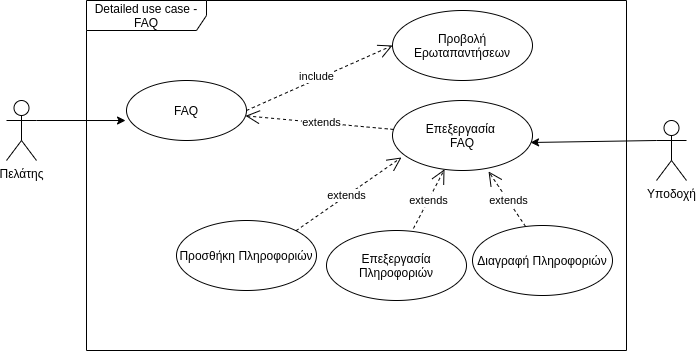
\includegraphics[width=0.8\textwidth]{Images/Low_level_use_case-FAQ}
	\caption{Low Level Use Case Diagram - FAQ}
	\label{Low_level_use_case - FAQ}
\end{figure}

\begin{figure}[H]
	\centering
	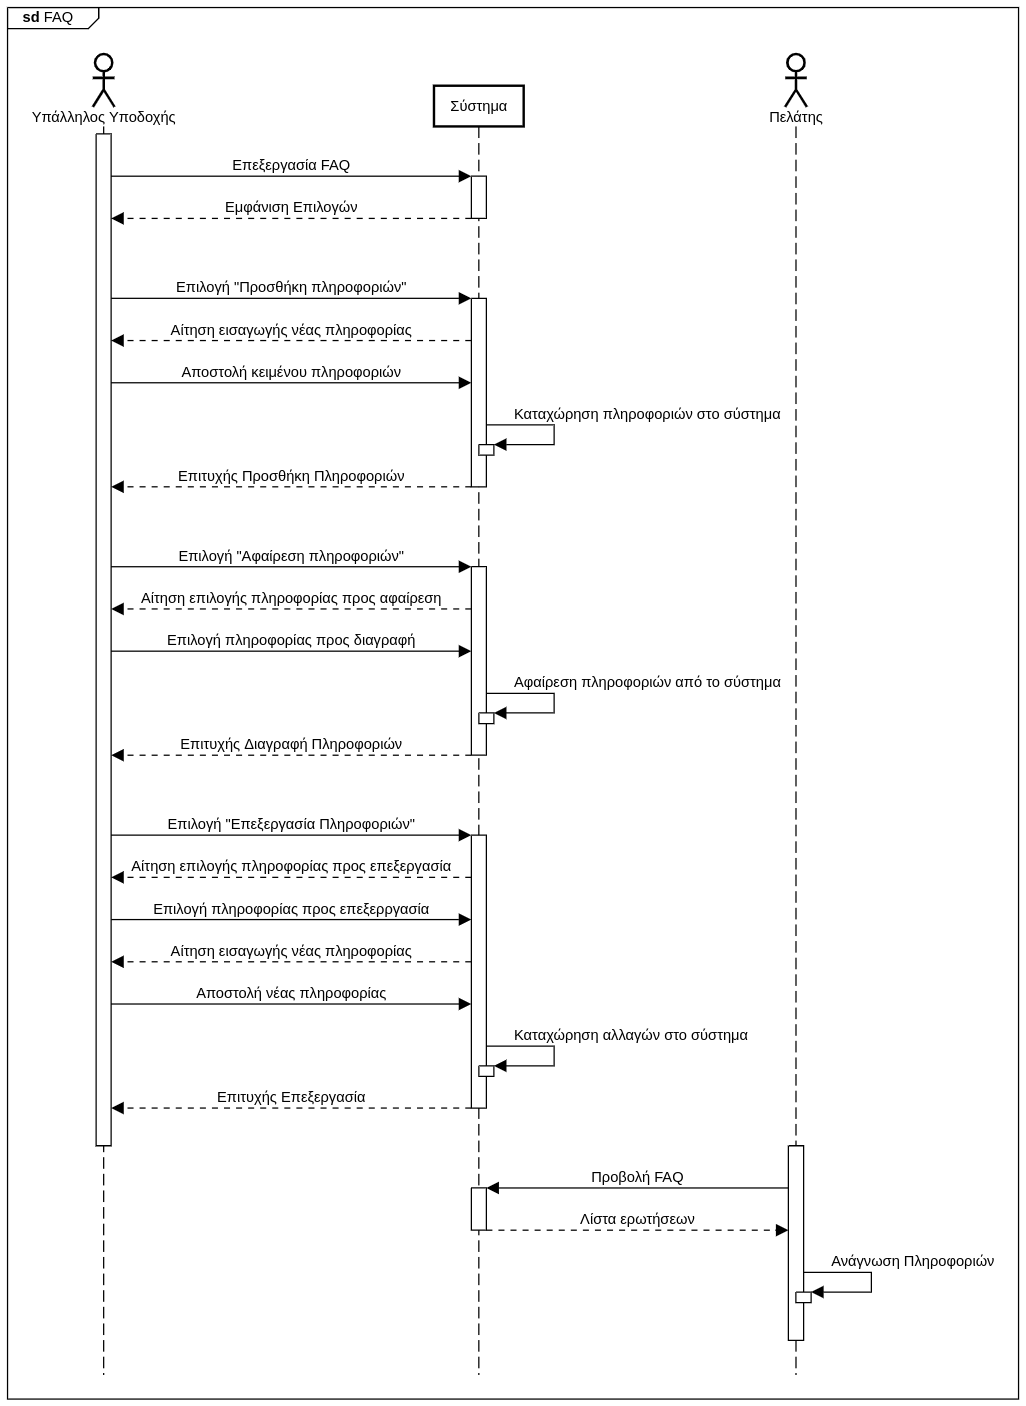
\includegraphics[width=0.6\textwidth]{Images/sequence-FAQ}
	\caption{Sequence diagram - FAQ}
	\label{Sequence_diagram - FAQ}
\end{figure}
\clearpage

\noindent 
Όσον αφορά την λειτουργία "Room Service" προβλέπεται μία διαδικασίες που μπορεί να εκπονηθεί.
Εμπλεκόμενοι σε αυτή τη λειτουργία είναι ο πελάτης και η καμαριέρα. Όσον αφορά τον πελάτη αρχικά,
γίνεται επιλογή της λειτουργίας "Room Service" από το κεντρικό μενού και στην συνέχεια από τον χρήστη
ζητείται η επιλογή του είδους γεύματος που επιθυμεί (Βραδινό ή Πρωινό). Μέσω αυτή της επιλογής, 
εμφανίζεται ο αντίστοιχος κατάλογος για το κάθε είδος, όπου ο χρήστης κάνει την/τις  επιλογή/ες του. 
Τέλος,  ζητείται η ώρα παράδοσης αυτού και εφόσον έχει ολοκληρώσει την παραγγελία του, το αίτημα 
του αποστέλλεται ενώ εμφανίζεται το αντίστοιχο μήνυμα εξόδου τύπου pop-up, ώστε ο πελάτης να 
γνωρίζει εάν το αίτημά του εγκρίθηκε ή απορρίφθηκε.  Μία από τις καμαριέρες που βρίσκο-\\νται σε 
βάρδια, δέχεται ειδοποίηση σχετικά με την παραγγελία και ελέγχει εάν οι προμήθειες επαρκούν. 
Ανάλογα με αυτές, μέσω την ειδοποίησης που έλαβε, εγκρίνει ή απορρίπτει το αίτημα του πελάτη. Σε  
περίπτωση απόρριψης, ο πελάτης έχει την δυνατότητα δημιουργίας νέας παραγγελίας εάν το επιθυμεί.
Τέλος, η συγκεκριμένη διαδικασία παρουσιάζει μέτρια προτεραιότητα καθώς αποτελεί σύγχρονη 
επικοινωνία μεταξύ χρηστών η οποία αποσκοπεί στην εξυπηρέτηση του πελάτη και γι αυτό 
είναι απαραίτητη η γρήγορη ενημέρωση τόσο του πελάτη όσο και της καμαριέρας. \\
\begin{figure}[H]
	\centering
	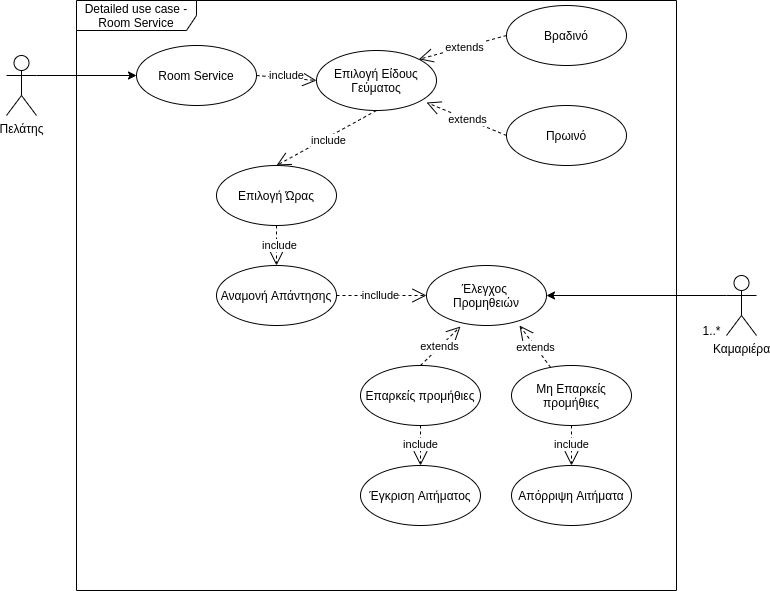
\includegraphics[width=1\textwidth]{Images/Low_level_use_case-Room service}
	\caption{Low Level Use Case Diagram - Room Service}
	\label{Low_level_use_case - Room Service}
\end{figure}
\begin{figure}[H]
	\centering
	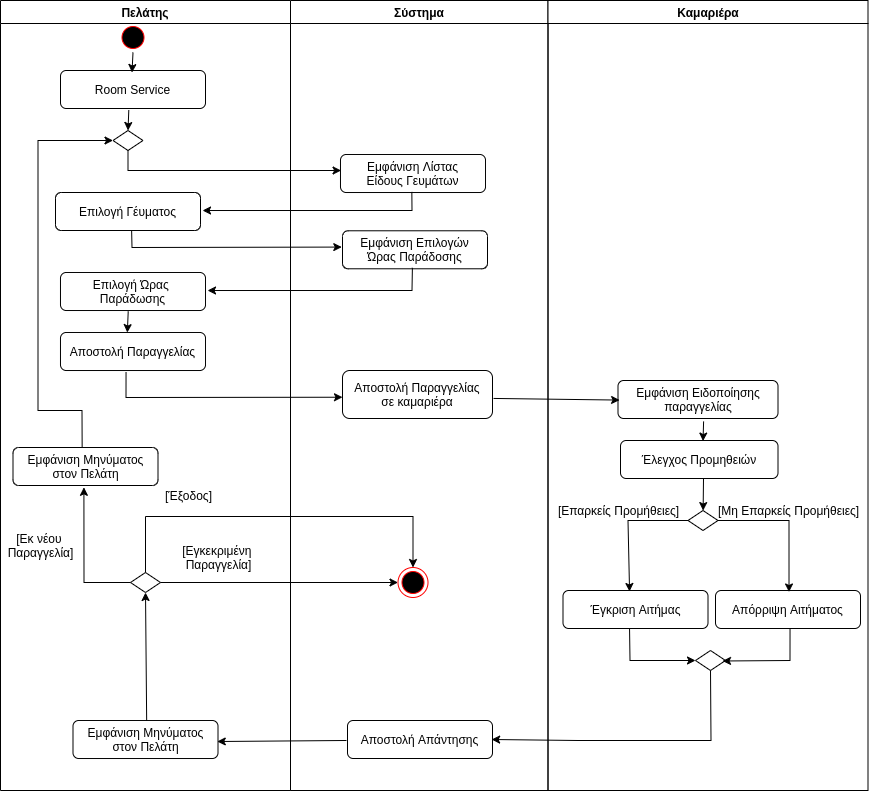
\includegraphics[width=1\textwidth]{Images/Activity-Room service}
	\caption{Activity Diagram - Room Service}
	\label{Activity - Room Service}
\end{figure}
\clearpage

\noindent
Όσον αφορά την λειτουργία "Επικοινωνία μέσω Chat" προβλέπονται δύο διαδικασίες που μπορεί να 
εκπονηθούν όπου εμπλεκόμενοι είναι ο πελάτης και ο υπάλληλος υποδοχής. Όσον αφορά τον πελάτη
αρχικά, γίνεται η επιλογή της λειτουργία "Επικοινωνία μέσω Chat", στο κεντρικό μενού, και στη 
συνέχεια το γραφικό περιβάλλον αλλάζει και γίνεται σαν ένα κοινό chat room.  Μέσω αυτού, ο 
πελάτης, έχει την δυνατότητα να στέλνει αλλά και να δέχεται μηνύματα από τον υπάλληλο 
υποδοχής,πραγματικό χρόνο. Με το πρώτο μήνυμα που στέλνει ο πελάτης, υπάλληλος υποδοχής 
έχει τη δυνατότητα να εισέλθει και αυτός το chat room μέσω της ειδοποίησης που δέχεται.  
Αντίστοιχη διαδικασία ακολουθείτε και από τον υπάλληλο υποδοχής στην περίπτωση που 
επιθυμεί να επικοινωνήσει με κάποιον πελάτη. Μοναδική διαφορά είναι πως όταν επιλέγει την 
λειτουργία "Επικοινωνία μέσω Chat", μία λίστα με όλα τα διαθέσιμα δωμάτια εμφανίζεται από την
οποία πρέπει να επιλέξει τον συνομιλητή του. Εφόσον γίνει αυτή η επιλογή, η διαδικασία είναι 
ακριβώς ίδια με πριν. Τέλος, η συγκεκριμένη διαδικασία παρουσιάζει υψηλή προτεραιότητα καθώς 
αποτελεί σύγχρονη επικοινωνία μεταξύ χρηστών και βασικός στόχος της είναι η αμεσότητα και η 
ταχύτητα για την καλύτερη εξυπηρέτηση των πελατών.\\ \\ \\ \\
\begin{figure}[H]
	\centering
	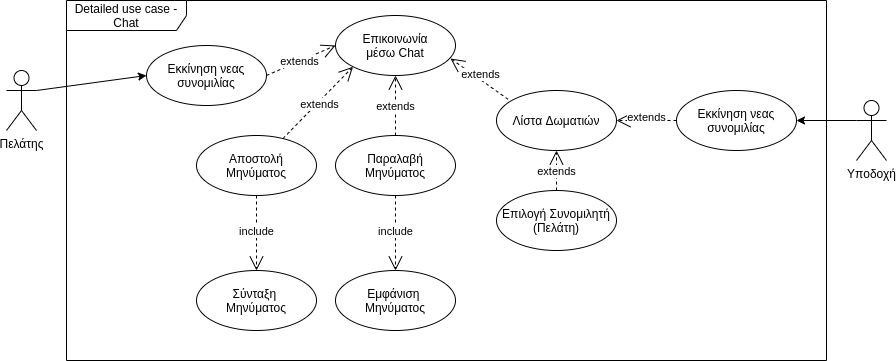
\includegraphics[width=1\textwidth]{Images/Low_level_use_case-Chat}
	\caption{Low Level Use Case Diagram - Chat}
	\label{Low_level_use_case - Chat}
\end{figure}
\begin{figure}[H]
	\centering
	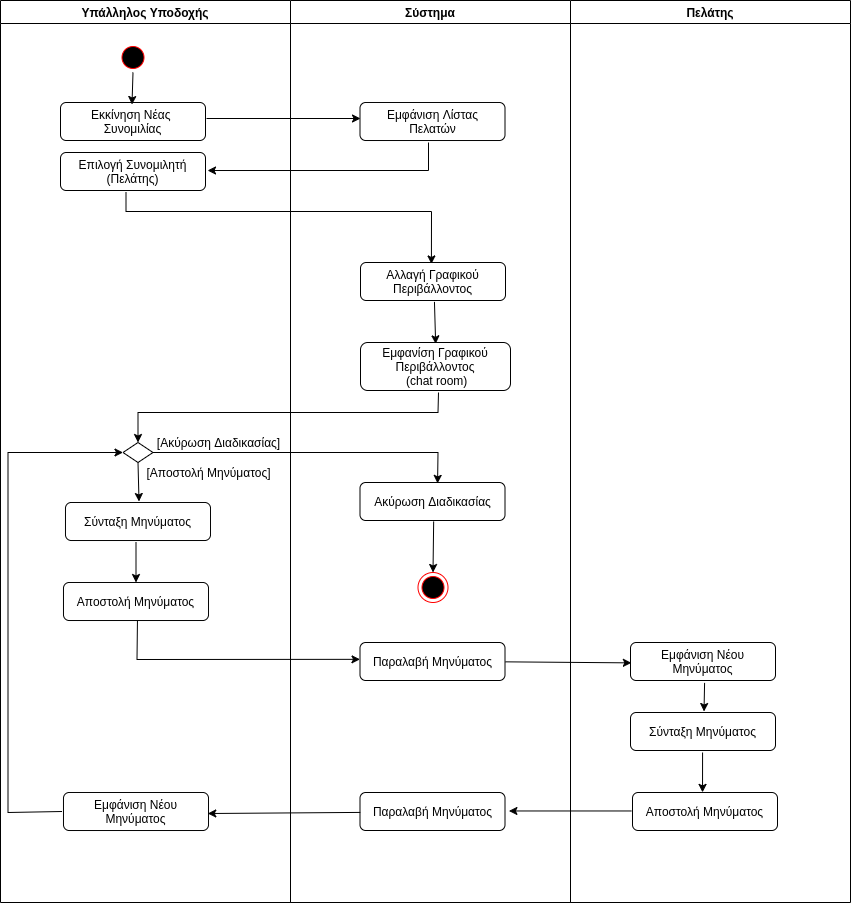
\includegraphics[width=1\textwidth]{Images/Activity-Chat}
	\caption{Activity Diagram - Chat}
	\label{Activity - Chat}
\end{figure}
\clearpage

\noindent
Όσον αφορά την λειτουργία "Καθαριότητα και Αναφορά Δωματίων" προβλέπεται μία διαδικασία
που μπορεί να εκπονηθούν όπου μοναδικός εμπλεκόμενος είναι η καμαριέρα. Αρχικά, γίνεται η 
επιλογή της λειτουργίας "Καθαρισμός Δωματίων" στο κεντρικό  μενού και στη συνέχεια ζητείται 
η προσθήκη του αριθμού δωματίου στο οποίο έγιναν οι απαραίτητοι έλεγχοι καθώς και τα 
προβλεπόμενα πρωτόκολλα καθαρισμού. Στη συνέχεια, εμφανίζεται μία λίστα με όλα τα αντικείμενα
τα οποία αναμένεται να υπάρ-\\χουν στο δωμάτιο στην οποία λίστα μπορεί να συμπληρώσει 
την ποσότητα κάθε αντικειμένου που βρέθηκε στο δωμάτιο. Σε περίπτωση που κάποιο 
αντικείμενο απουσιάζει ή παρουσιάζεται έλλειψη, δηλαδή δηλώνεται μικρότερος αριθμός από 
τον αναμενόμενο,αυτό προστίθεται μέσω έτοιμου κώδικα σε ένα αρχείο τύπου csv, ώστε να 
μπορεί να γίνει η αντίστοιχη παραγγελία στους προμηθευτές, από την υπάλληλο υποδοχής.
Αυτή η διαδικασία επαναλαμβάνεται έως ότου η καμαριέρα συμπληρώσει τον προβλεπόμενο 
αριθμό δωματίων που έχει αναλάβει. Τέλος, η συγκεκριμένη διαδικασία παρουσιάζει χαμηλή 
προτεραιότητα καθώς κατά την εκπόνησή της γίνεται συμπλήρωση μίας λίστας η οποία θα 
επεξεργαστεί από το σύστημα εσωτερικά και ο μόνος που θα αλληλεπιδράσει με την έξοδο
που πιθανώς να δημιουργηθεί, είναι η υπάλληλος υποδοχής κάτι το οποίο  όμως θα γίνει σε 
μεταγενέστερο χρόνο.\\\\
\begin{figure}[H]
	\centering
	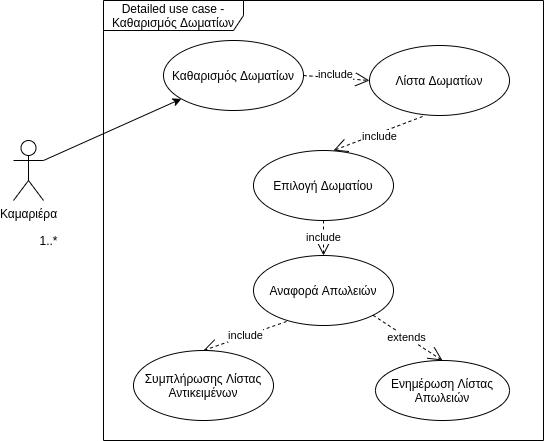
\includegraphics[width=1\textwidth]{Images/Low_level_use_case-Room cleaning}
	\caption{Low Level Use Case Diagram - Καθαρισμός Δωματίων}
	\label{Low_level_use_case - Room cleaning}
\end{figure}

\begin{figure}[H]
	\centering
	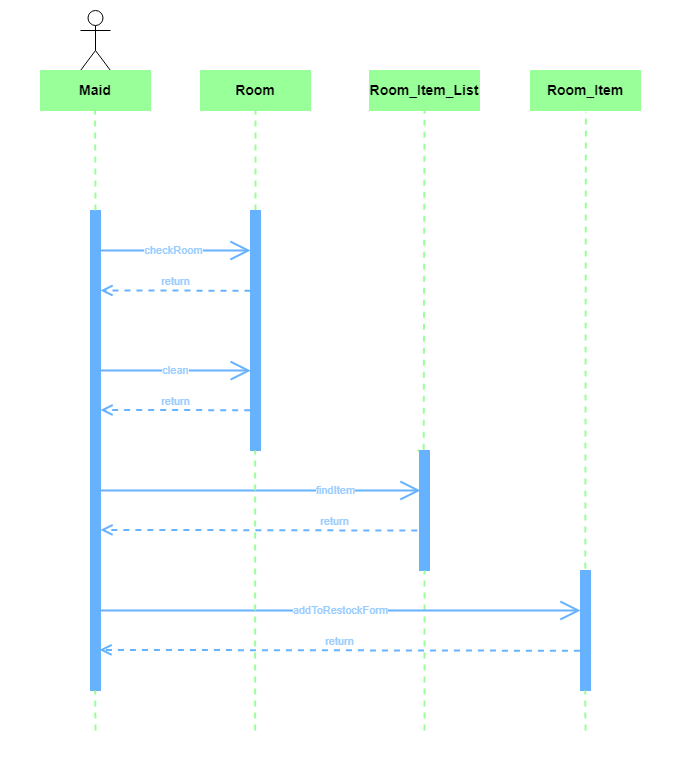
\includegraphics[width=1\textwidth]{Images/Sequence-Room cleaning}
	\caption{Low Level Use Case Diagram - Καθαρισμός Δωματίων}
	\label{Activity- Room cleaning}
\end{figure}

\section{Μή Λειτουργικές Απαιτήσεις}
